\section{Investigaciones previas}
\subsection{Investigación de algoritmos de similitud}
Para mejorar la experiencia del usuario en \loopweb, se analizaron diferentes algoritmos de similitud utilizados en redes sociales. Estos algoritmos permiten establecer conexiones y recomendaciones basadas en intereses y afinidades entre usuarios.

\begin{enumerate}
    \item \textbf{Similaridad de Jaccard}: Este algoritmo utiliza la teoría de conjuntos, usando la unión e intersección, si los conjuntos tienen todas sus componentes similares, su índice de similitud será $1$, en cambio si no hay ningún componente similar el índice será $0$. Este índice se calcula: \[J(A,B)=\frac{|A\cap B|}{|A\cup B|}\]
        \begin{figure}[!ht]
            \centering
            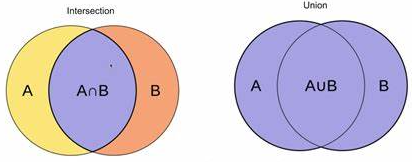
\includegraphics[width=0.4\textwidth]{./src/images/Indice de Jaccard.png}
            \caption{Índice de Jaccard}
            \label{fig:indicejaccard}
        \end{figure}

    \item \textbf{Similaridad del Coseno}: Mide la semejanza entre dos vectores calculando el coseno del ángulo entre estos: \[\text{Similitud}(U,V)=\frac{\vec{U}\circ\vec{V}}{|\vec{U}|\cdot|\vec{V}|}\]
    \item \textbf{Similaridad de Pearson}: Este algoritmo mide la relación \textbf{lineal} entre dos variables, que tan estrechos se alinean los puntos a lo largo de una línea recta en una gráfica de dispersión. El coeficiente varía de $-1$ a $+1$, donde $-1$ indica una correlación negativa perfecta, $+1$ representa una correlación positiva perfecta, y $0$ sugiere una relación lineal entre las variables. \[r=\frac{\frac{\sum(x_{i}\cdot y_{i})}{N}-(\overline{x}\cdot \overline{y})}{\sigma_{x}\cdot\sigma_{y}}\]
    \item \textbf{Coeficiente de Dice}: También conocido como índice de Sørensen-Dice, es una herramienta estadística que está destinada a ser aplicada en datos para ver la presencia o ausencia de valores. Una puntuación de 0 significa que no hay superposición entre los dos conjuntos, mientras que una puntuación de 1 significa que son idénticos. \[\text{Similaridad }(A,B)=2\frac{|A\cap B|}{|A|+|B|}\]
    \item \textbf{Vecinos comunes}: Es una técnica simple que mide la similitud entre nodos (o usuarios) en función de los vecinos compartidos, este identifica los vecinos de cada nodo, luego calcula la intersección de vecinos compartidos y usa metricas de conteo para determinar la similitud.
    \item \textbf{Índice de Adamic-Adar}: Es una métrica basada en vecinos comunes pero se enfoca mas en los nodos pocos comunes, es más sofisticado que el simple conteo de vecinos comunes porque considera la rareza de los nodos comunes.
\end{enumerate}

\subsection{Analisis de las redes sociales}
Para crear una simulación de una red social es necesario conocer el funcionamiento de otras redes sociales comunes en nuestros tiempos, es por esta razón que se realizó un análisis de las redes sociales más populares y aquello que pueden aportar a nuestra experiencia en \loopweb.
\begin{enumerate}
    \item \textbf{Bluesky}: Es una plataforma de redes sociales descentralizada que se fundó como una iniciativa de investigación como parte de Twitter en 2019. \textbf{Bluesky} es especial porque combina las ventajas de la descentralización (propiedad de datos, flexibilidad, diversidad de comunidades) con la facilidad de uso de las plataformas centralizadas. Alguna de sus características más destacables son:
        \begin{itemize}
            \item Permite a sus usuarios personalizar el contenido que desean ver, es un tipo de visualización de contenido en el que las publicaciones se ordenan según la relevancia y el interés para el usuario, en lugar de la cronología.
            \item Los post son mas cortos, cuenta con un limite de $300$ caracteres, y pueden incluir fotos y videos.
        \end{itemize}
    Uno de los puntos mas fuertes de Bluesky es el feed, ya que permite tener una experiencia mas personalizada al navegar por la red social, se puede crear un propio feed que permite un mejor viaje a través de la red social, eligiendo distintos contenidos para visualizar.

    \item \textbf{Spotify}: Es una plataforma de música y podcasts digitales que da acceso a millones de canciones. Los creadores de esta red social saben que no hay dos oyentes iguales, por lo que la experiencia para cada usuario y muchas de las recomendaciones, son personalizadas.
    Algunas recomendaciones se basan en la selección editorial, como una playlist de música creada por editores musicales. Otras recomendaciones se adaptan al gusto único de cada oyente, como una playlist personalizada.

    \item \textbf{Facebook}: Es la principal red social que existe en el mundo. Una red de vínculos virtuales, cuyo principal objetivo es dar un soporte para producir y compartir contenidos.

    Las sugerencias de amistad se basan en factores como: \textbf{amigos en común}, por medio de ciudad, escuela o trabajo, pertenecer a un mismo grupo, etiquetas en publicaciones, contactos vinculados. Sin embargo las recomendaciones también se basan en la ubicación (no precisa) del usuario, su idioma, su edad y sus perfiles seguidos.

    \item \textbf{Youtube}: Es un sitio web dedicado a compartir videos, presenta una variedad de clips, programas de television, videos musicales, gameplays, videoblogs. Las recomendaciones de contenido de esta aplicación se centran en: Encuestas, Intereses e interacciones.

    \item \textbf{TikTok}: Permite crear, editar y subir vídeos propios o de terceros inicialmente con una duración máxima de un minuto a los que se les incluyen fondos musicales o sonidos.
    El algoritmo de TikTok es una fórmula patentada que determina qué videos se muestran a cada usuario. Los principales factores que influyen en el algoritmo de TikTok son las interacciones de los usuarios, la información de los videos, la configuración del dispositivo y la cuenta.
    \item \textbf{Instagram}: Es una red social principalmente visual, donde un usuario puede publicar fotos, videos e historias de corta duracion. En Instagram, no hay un solo algoritmo que decide lo que se ve, ya que cada parte de la app (el feed, la sección `Explorar' y los Reels) tiene su propio sistema de clasificación según cómo es usado. Actualmente, el algoritmo de Instagram da prioridad a las \textbf{publicaciones más recientes}.
\end{enumerate}

\subsection*{¿Que se aplicó de estas aplicaciones a \loopweb?}
Muchas de estas redes sociales tienen algoritmos y características importantes, algunas de las ideas que tomó \loopweb de estas aplicaciones son:
\begin{itemize}
    \item Feed personalizado (como Bluesky)
    \item Personas que quizás conozcas (como Facebook e Instagram)
    \item Limite de caracteres (como Bluesky)
    \item Gestión y enlaces entre usuarios
\end{itemize}